\section{Finite samples}\label{sec:finite}

Limits describe large samples. This section answers two questions for the sample sizes people use: how large is the worst-case size of the standard test at a given $n$, and which cutoff keeps the level at that $n$. Every statement here is made at the listed values of $n$ only; we prove nothing about monotonicity in $n$.

\subsection{The size of the standard test}
At each of 21 sample sizes from $n=4$ to $n=1000$, and at the levels 10, 5 and 1 percent, we enclosed the worst-case size $S_n(\alpha)$ in an interval. The 63 intervals hold jointly with confidence at least $0.991$.

The lower end of each interval is witnessed by a specific unimodal law. We found the law by search, and then re-estimated its rejection rate on fresh random draws, so the search cannot bias the estimate; an exact binomial bound turns the estimate into a lower confidence limit.

The upper end comes from one computation on uniform samples, which by \cref{thm:envelope} covers every law at once. For each simulated uniform sample we bound its distance to $K_u$ over all turning points $u$, and the sample counts as non-rejecting only when a certified upper bound on that distance falls strictly below the cutoff.

\Cref{fig:worstsize} shows them. At every listed $n$ and level the size exceeds the nominal level. At $n=1000$ the 5 percent test has worst-case size between 28.0 and 34.2 percent, which agrees with the asymptotic interval of \cref{thm:worst}. At small $n$ the intervals are wide, 27 to 57 points for $n$ between 5 and 12, so the exact worst-case size there is not known. A simpler statement holds at every $n$: with the same joint confidence, the running example $W(0.1,0.005)$ is rejected more often than the nominal rate at each of the 997 integers from 4 to 1000 and at all three levels. At $n=50$, for example, its rejection rates are 3.9, 13.5 and 23.2 percent at the 1, 5 and 10 percent levels.

\begin{figure}[t]
\centering
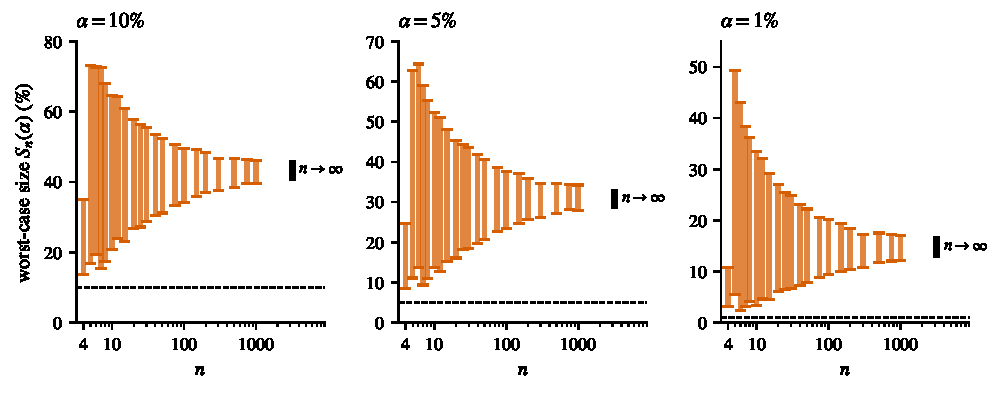
\includegraphics[width=\linewidth]{figs/fig4_worst_size.pdf}
\caption{The worst-case size of the standard dip test exceeds the nominal level at every sample size shown, and at $n=1000$ its enclosure overlaps the asymptotic interval. Orange bars: enclosures at 21 sample sizes. They hold jointly with confidence at least $0.991$, and their lower ends at $n=4$ are exact. Black bars: the asymptotic interval of \cref{thm:worst}. Dashed lines: nominal level.}
\label{fig:worstsize}
\end{figure}

\subsection{Certified cutoffs}
\Cref{thm:envelope} also turns the search for a valid cutoff into a computation on uniform samples. For a candidate cutoff $d$ at a given $n$ we simulate uniform samples, compute the distance to $K_u$ over each block of turning points by an exact linear program, and accept $d$ when the binomial upper bound on the exceedance rate is at most $\alpha$ in every block, after a Bonferroni correction over all candidates and sample sizes in the run. \Cref{tab:cutoffs} lists the result, and \cref{fig:cutoffs} compares the certified cutoffs with the uniform quantiles that the standard test uses.

\begin{table}[t]
\centering
\small
\caption{Certified dip cutoffs. Rejecting when $D_n\ge d$ has size at most $\alpha$ over all continuous unimodal laws at the listed $n$. Cutoffs are given on the scale $\sqrt n\,d$, except at $n=4$, where $d$ itself is shown with the certified bound on the size. The false-certification probability is at most $0.001$ for the first two rows and at most $0.02$ for the third.}
\label{tab:cutoffs}
\begin{tabular}{p{2.9cm}ccc}
\toprule
$n$ & $\alpha=10\%$ & $\alpha=5\%$ & $\alpha=1\%$ \\
\midrule
4 & $0.2335$ ($\le9.62\%$) & $0.2420$ ($\le4.62\%$) & $0.2488$ ($\le0.68\%$) \\
8 to 49, every $n$ & $\rho\times0.667$ & $\rho\times0.7313$ & $\rho\times0.8585$ \\
50, 100, 200, 400, 800, 1600 & & $0.7315$ & $0.86$ ($n\le800$); $0.87$ ($n=1600$) \\
\bottomrule
\end{tabular}
\par\smallskip
\raggedright\footnotesize For $8\le n\le49$ the certified cutoff is $\rho$ times the lower end of the bracket for $c_\alpha$, divided by $\sqrt n$. The factor $\rho$ was chosen from the fixed ladder $0.900,0.905,\dots,0.995$ by a rule set in the protocol; the certified values lie between $0.945$ and $0.995$ and depend on $n$ and $\alpha$, and the full list is in the supplement. In five of these 126 cases ($n=8,10,11$ at 1 percent and $n=9$ at 5 and 1 percent) the certified cutoff exceeds the largest possible dip (\cref{lem:maxdip}), so the test never rejects there.
\end{table}

\begin{figure}[t]
\centering
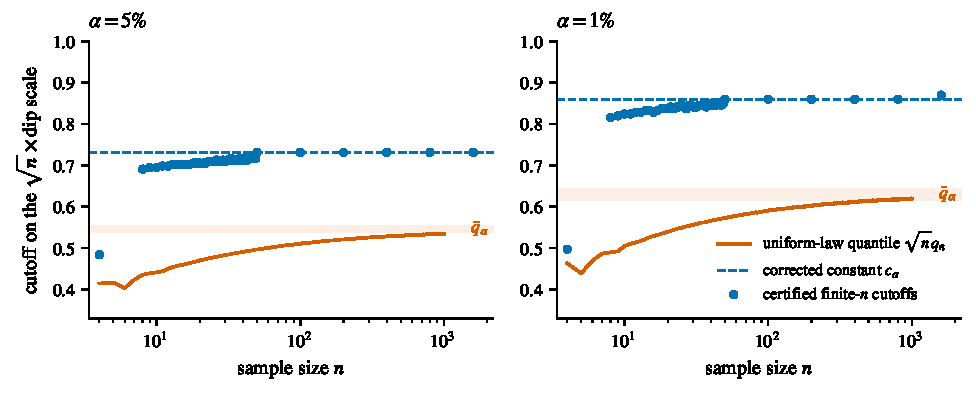
\includegraphics[width=\linewidth]{figs/fig5_cutoffs.pdf}
\caption{Valid cutoffs lie above the uniform quantiles that the standard test uses, at every sample size. Cutoffs are shown on the scale $\sqrt n\times$dip. Orange: the uniform quantile $\sqrt n\,q_n$ used by the standard test, rising towards $\qbar_\alpha$ (shaded bracket). Blue dashed: the corrected constant $c_\alpha$. Blue dots: certified cutoffs from \cref{tab:cutoffs}. At every $n$ shown, the certified cutoff lies above the uniform quantile.}
\label{fig:cutoffs}
\end{figure}

Three features of the table matter in practice. At $n=4$ the certified cutoffs lie just below $1/4$, the largest dip four points can have, while $c_\alpha/\sqrt4$ exceeds $1/4$ at every level, so the asymptotic cutoff could never reject at $n=4$. For $8\le n\le49$ the certified cutoffs lie a little below $c_\alpha/\sqrt n$, so each certified test rejects whenever the asymptotic one does and has at least its power; as a by-product, $c_\alpha/\sqrt n$ itself has size at most $\alpha$ at all 126 of these $(n,\alpha)$ pairs. At the six listed sizes from 50 to 1600, the rounded value $0.7315$ is certified at 5 percent. The best laws we found reach only 1.6 to 3.3 percent at that cutoff, so the certified cutoffs are valid but we do not claim that they are the smallest valid ones. Two cutoffs that are valid at every $n$ are already known, and both are larger: half the Kuiper distance of Davies and Kovac \cite{DK04}, $0.874/\sqrt n$ at 5 percent, and the Dvoretzky--Kiefer--Wolfowitz bound with Massart's constant \cite{Massart90}, $1.3582/\sqrt n$ at 5 percent and $1.6277/\sqrt n$ at 1 percent.

\subsection{Very small samples}
At $n=4$ the dip has a closed form. If $s_1,s_2,s_3$ are the gaps between the four ordered observations, Hartigan and Hartigan \cite[p.~73]{HH85} show that $D=T/(4(T+1))$ with $T=\max\{1,\,s_2/\max(s_1,s_3)\}$. Under the uniform law $P(T\ge r)=2/((r+1)(r+2))$ for $r>1$, so the exact uniform critical value is $q_4(1-\alpha)=r_\alpha/(4(r_\alpha+1))$, where $(r_\alpha+1)(r_\alpha+2)=2/\alpha$. For a step law the rejection probability is then the volume of a polytope, which we compute in rational arithmetic. For the running example the exact rates, truncated to four decimals, are $10.6639$, $5.5465$ and $1.2908$ percent at the 10, 5 and 1 percent levels, only a small excess at this sample size. Other laws do worse. Laws built from parts on widely separated scales give
\[
S_4(\alpha)\ \ge\ 13.7461,\ 8.5962,\ 3.2638\ \text{percent at}\ \alpha=10,\ 5,\ 1\ \text{percent},
\]
and we conjecture that these values are the exact worst case. The Monte Carlo upper bounds are 34.93, 24.60 and 10.70 percent. At $n=4$, then, the flat shoulder with a thin top is not the worst shape.

Small samples also have a hard ceiling on the dip, which explains the five cases in \cref{tab:cutoffs} where the certified test never rejects.

\begin{lemma}[largest possible dip]\label{lem:maxdip}
For every $n\ge1$ and every data set, ties allowed, $D(F_n)\le\lfloor n/2\rfloor/(2n)$. The bound is attained when $\lfloor n/2\rfloor$ points sit at one value and the rest at another.
\end{lemma}
\begin{proof}
Let $k=\lfloor n/2\rfloor$, $\varepsilon=k/(2n)$, let $m$ be the $(k+1)$-th order statistic and $R>0$ the sample range (if $R=0$ the dip is $0$). For $T\ge R$ let $G_T$ put mass $\varepsilon$ evenly on $[m-T,m]$, an atom $1-2\varepsilon$ at $m$, and mass $\varepsilon$ evenly on $[m,m+T]$; it is unimodal with mode $m$. Left of $m$ we have $F_n\le k/n=2\varepsilon$, and from $m$ on $F_n\ge(k+1)/n\ge1-2\varepsilon$, and comparing the two functions gives $\sup|F_n-G_T|\le\varepsilon(1+R/T)$. Let $T\to\infty$.
\end{proof}

The value $1/4$ for even $n$ is noted in Mächler's vignette \cite{Maechler}; the odd-$n$ value $(n-1)/(4n)$ is elementary, and we did not find it stated elsewhere.
